% Semantic Assistants - http://www.semanticsoftware.info/semantic-assistants
%
% This file is part of the Semantic Assistants architecture.
%
% Copyright (C) 2009, 2010, 2011 Semantic Software Lab, http://www.semanticsoftware.info
% The Semantic Assistants architecture is free software: you can
% redistribute and/or modify it under the terms of the GNU Affero General
% Public License as published by the Free Software Foundation, either
% version 3 of the License, or (at your option) any later version.
%   
% This program is distributed in the hope that it will be useful,
% but WITHOUT ANY WARRANTY; without even the implied warranty of
% MERCHANTABILITY or FITNESS FOR A PARTICULAR PURPOSE.  See the
% GNU Affero General Public License for more details.
% 
% You should have received a copy of the GNU Affero General Public License
% along with this program.  If not, see <http://www.gnu.org/licenses/>.

\chapter{Extension for Mozilla Firefox and Mozilla Thunderbird} 

The Mozilla extension allows users to use Semantic Assistants in Mozilla Firefox and Mozilla Thunderbird and to leverage the \sa architecture within those applications. It is built on the extension platform that shared by Mozilla Firefox and Mozilla Thunderbird. Hence, it is a single extension that is compatible with both applications. The Mozilla extension aims to take the capabilities provided by Semantic Assistants and integrate them within the workflow of web browsing and of email reading and management. 

\section{Features}
\label{subsec:mozilla_features}

\subsection{User Interface Elements}
When the \sa Mozilla extension is installed, some new UI elements are added to the interface of the application. Firstly, a new ``Semantic Assistants" menu is added on the menu bar. Secondly, a new toolbar button is added to the primary toolbar of the application. (This toolbar button may be removed or relocated using Firefox/Thunderbird's built-in customization capabilities.) The toolbar button is actually a ``menu button," i.e., the left part is a button, and the right part opens a menu when clicked. Thirdly, a menu item is added to the contextual (right-click) menu of the principal content area of the application, that is, the browsing area in Firefox and the message body pane in Thunderbird. Lastly, a sidebar, which can be opened and closed, is added to the main window of the application. 

\paragraph{The ``Semantic Assistants" menu.} The ``Semantic Assistants" menu is 
located on the menu bar and opens a menu with the following three menu items: 
\begin{itemize} 
  \item Available Assistants... 
  \item Semantic Assistants Sidebar 
  \item Global Settings... 
\end{itemize} 

The ``Semantic Assistants" menu is shown in Figure~\ref{fig:mozilla_features_toolbar_menu_button}. 

\begin{figure}[htb]
  \centering
  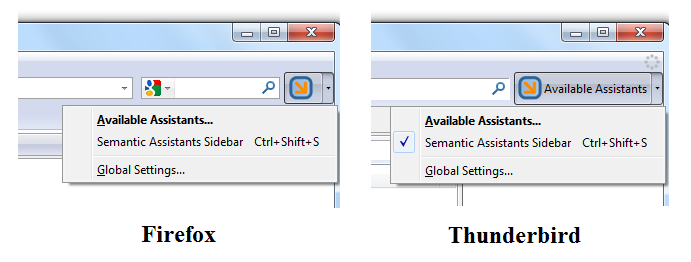
\includegraphics[width=0.8\textwidth]{pictures/mozilla_features_toolbar_menu_button.png}
  \caption{The toolbar menu button in Firefox and Thunderbird}
  \label{fig:mozilla_features_toolbar_menu_button}
\end{figure}

\paragraph{The ``Available Assistants" toolbar menu button.} The ``Available Assistants" menu button is located on the toolbar. The left side is a button and executes the ``Available Assistants" command (further elaborated later). Clicking the right side opens a menu that is identical to the ``Semantic Assistants" menu. 

\paragraph{The ``Available Assistants..." contextual menu item.} The ``Available Assistants" menu item appears on the contextual (right-click) menu of the main browsing area/page content area in Firefox and in the message body area in Thunderbird. Like the toolbar button, it also invokes the ``Available Assistants" command. 

\paragraph{The ``Semantic Assistants Sidebar".} The ``Semantic Assistants Sidebar" appears on the left side of the main window in Firefox and on the right side of the main window in Thunderbird. (The discrepancy is explained as follows. Firefox has built-in support for adding sidebars, and these appear on the left side of the main browsing window. Thunderbird, on the other hand, has no sidebars. Furthermore, the main inbox tab in Thunderbird already has a folder pane on the left side of the window. Hence, a custom sidebar was added, and it was placed on the right side of the main window.) 

The ``Semantic Assistants Sidebar" displays the results obtained from a service invocation to a Semantic Assistant. The following button in the Sidebar operate on the results: 
\begin{itemize} 
  \item \emph{Expand all}: Expands nodes of the results tree by one level.
  \item \emph{Collapse all}: Collapses all nodes of the results tree.
  \item \emph{Underline all}: Underlines all results in the tree in the page/message.
  \item \emph{Underline none}: Clears all the underlining in the page/message.
  \item \emph{Find previous underlined item}: Selects (highlights) the previous underlined text in the page/message.
  \item \emph{Find next underlined item}: Selects (highlights) the next underlined text in the page/message.
\end{itemize} 
The ``Semantic Assistants Sidebar" can be opened using the following ways: 
\begin{itemize} 
  \item \emph{Semantic Assistants} menu $\rightarrow$ \emph{Semantic Assistants Sidebar}
  \item \emph{Available Assistants} toolbar button menu $\rightarrow$ \emph{Semantic Assistants Sidebar}
  \item (in Firefox) \emph{View} menu $\rightarrow$ \emph{Sidebar} $\rightarrow$ \emph{Semantic Assistants Sidebar}
  \item (in Thunderbird) \emph{View} menu $\rightarrow$ \emph{Layout} $\rightarrow$ \emph{Semantic Assistants Sidebar}
  \item the keyboard shortcut \emph{Ctrl Shift S}
\end{itemize} 

The ``Semantic Assistants Sidebar" dialog is shown in Figure~\ref{fig:mozilla_features_sidebar}. 

\begin{figure}[htb]
  \centering
  % \includegraphics[width=0.8\textwidth]
  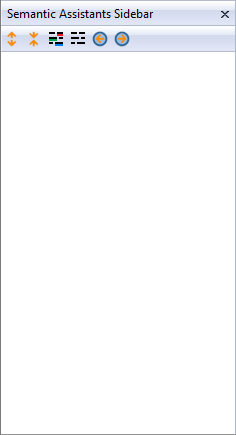
\includegraphics[totalheight=0.5\textheight]{pictures/mozilla_features_sidebar.png}
  \caption{The ``Semantic Assistants Sidebar" in Firefox and Thunderbird}
  \label{fig:mozilla_features_sidebar}
\end{figure}

\paragraph{The ``Global Settings" dialog.} The ``Global Settings" dialog allows the user to configure certain settings for the extension. These settings include:
\begin{itemize} 
  \item \emph{Server settings}: The user may choose to use the default defined server or to specify a custom server address. 
  \item \emph{Script settings}: The processing of the results is handled by a script run in Firefox/Thunderbird. If there are a lot of results or the page/message is long, the script may run for a long time. Firefox/Thunderbird has the built-in capability to prompt the user when a script has run for a given amount of time. By default, this amount of time is 20 seconds. The user may change this period if desired. Setting this setting to 0 signifies that the script will run forever. (Doing so, however, is not recommended, as the script may run for a very long time, and the only way to cancel would be to kill the whole application.)
\end{itemize} 
The ``Global Settings" dialog can be opened using the following ways: 
\begin{itemize} 
  \item \emph{Semantic Assistants} menu $\rightarrow$ \emph{Global Settings...}
  \item \emph{Available Assistants} toolbar button menu $\rightarrow$ \emph{Global Settings...}
\end{itemize} 

The ``Global Settings" dialog is shown in Figure~\ref{fig:mozilla_features_global_settings}. 

\begin{figure}[htb]
  \centering
  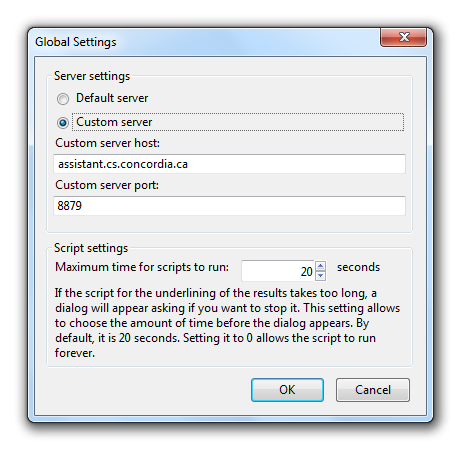
\includegraphics[width=0.8\textwidth]{pictures/mozilla_features_global_settings.png}
  \caption{The ``Global Settings" dialog in Firefox and Thunderbird}
  \label{fig:mozilla_features_global_settings}
\end{figure}

\subsection{Invoking a Semantic Assistant}
When the ``Available Assistants" command is invoked (either using the menu item in the ``Semantic Assistants" menu or in the menu of the toolbar button), a dialog entitled ``Available Semantic Assistants Services" appears (shown in Figure~\ref{fig:mozilla_features_available_assistants_dialog}), listing all available services from the server along with descriptions of each service. Upon the selection of a service, the extension sends the user-selected text in the page/message or, if text no selection was made, the whole text content of the page/message.

\begin{figure}[htb]
  \centering
  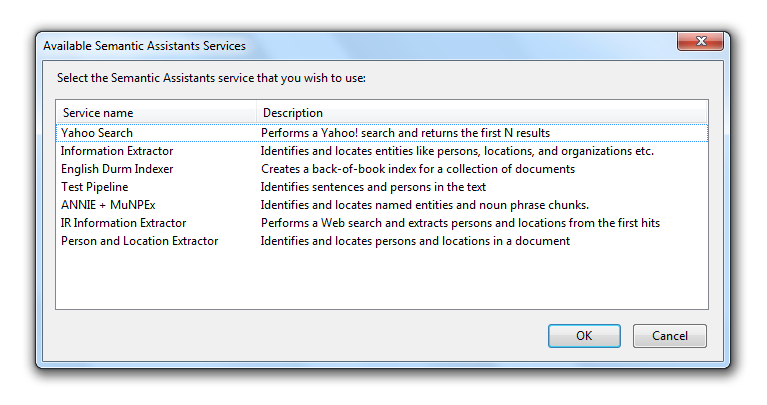
\includegraphics[width=1\textwidth]{pictures/mozilla_features_available_assistants_dialog.png}
  \caption{The ``Available Semantic Assistants Services" dialog in Firefox and Thunderbird}
  \label{fig:mozilla_features_available_assistants_dialog}
\end{figure}

When the results are returned by the server, two things happen. Firstly, the results are underlined in the page/message directly in the browsing area/message content area. Secondly, the ``Semantic Assistants Sidebar" is opened if it is not already so and displays the results. 

\subsection{Viewing the Results}
The results from the service invocation are underlined directly in the content of the page/message. The underlining is color-coded by annotation type to allow for better visual distinction. 

The results are also displayed in the ``Semantic Assistants Sidebar" in a tree format, grouped by annotation type, then by occurrences of a same word/phrase. 

The controls/buttons in the ``Semantic Assistants Sidebar" (mentioned previously in the ``User Interface Elements" section) can be used to manipulate the results tree, to underline all or no results and to go to the previous/next underlined result in the page/message.

Clicking on a node in the results tree will underline in the page/message the result or results represented by the node and all children of the node. For instance, if a leaf node of the tree is clicked in the Sidebar, the one result represented by that node is underlined. If an inner node of the tree is clicked in the Sidebar, then all the results represented by that node and all its child nodes are underlined. The ``Find previous underlined item" and ``Find next underlined item" buttons in the Sidebar will navigate only the currently underlined results. All put together, this allows to display precise subsets of the results, and to navigate through the occurrences of these results. 

The display of results within Firefox and Thunderbird is shown in Figure~\ref{fig:mozilla_features_firefox_window} and Figure~\ref{fig:mozilla_features_thunderbird_window_message_tab}.

\begin{figure}[htb]
  \centering
  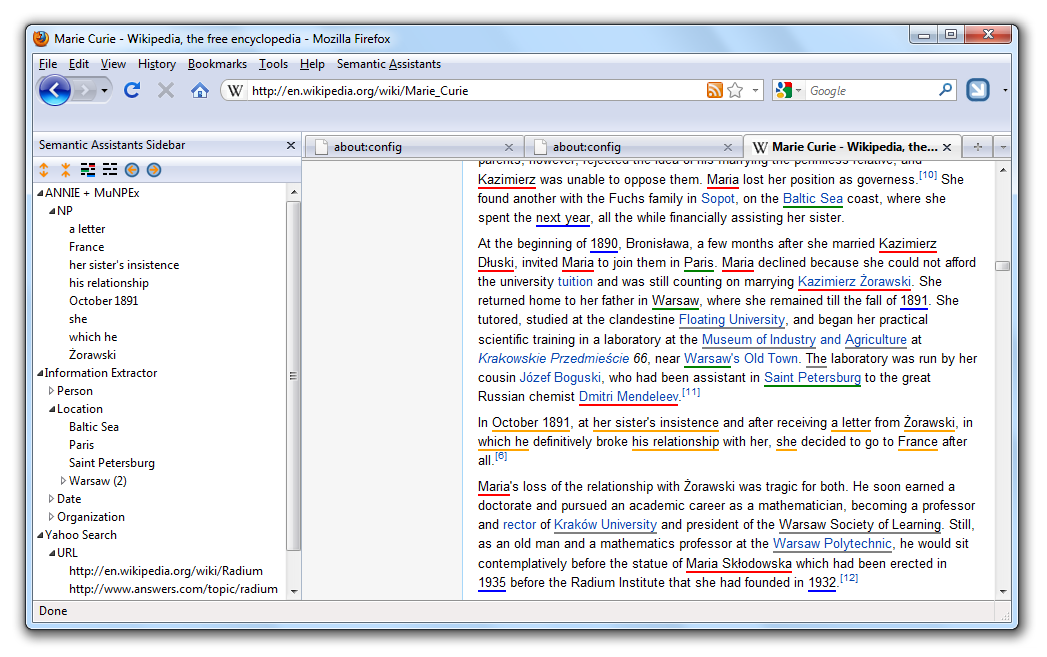
\includegraphics[width=0.95\textwidth]{pictures/mozilla_features_firefox_window.png}
  \caption{Results from a service invocation in Firefox}
  \label{fig:mozilla_features_firefox_window}
\end{figure}

\begin{figure}[htb]
  \centering
  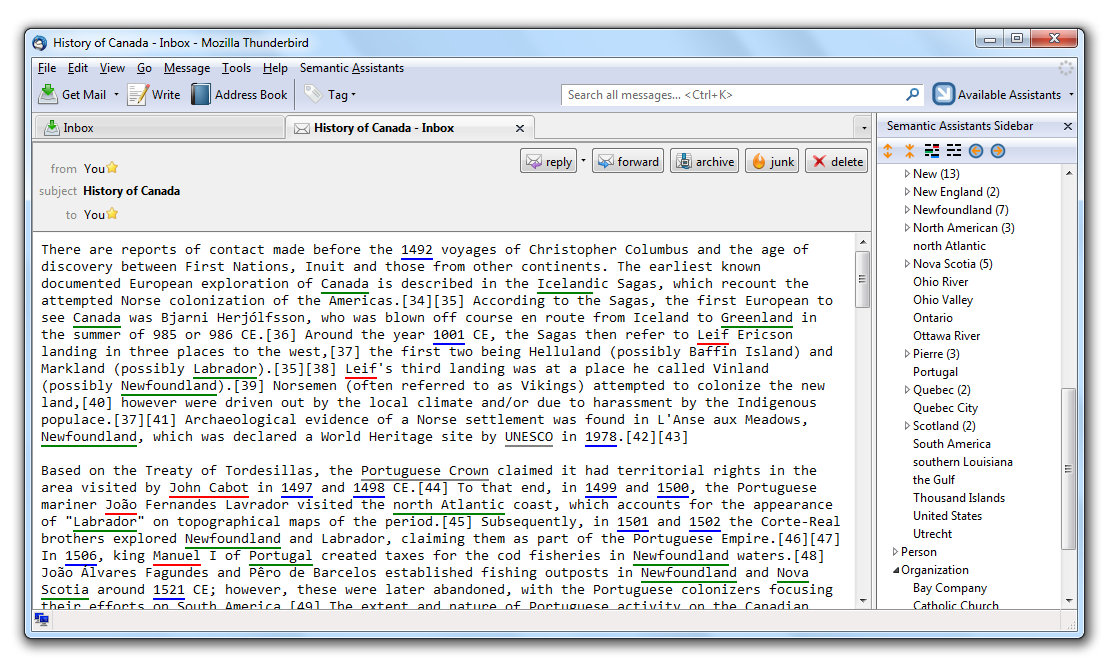
\includegraphics[width=0.95\textwidth]{pictures/mozilla_features_thunderbird_window_message_tab.png}
  \caption{Results from a service invocation in Thunderbird}
  \label{fig:mozilla_features_thunderbird_window_message_tab}
\end{figure}

\section{Installation}
\label{subsec:mozilla_installation}
The Mozilla extension comes in the form of a file with a .xpi extension. The .xpi file is installed in the standard manner in which extensions are installed in Mozilla Firefox and Mozilla Thunderbird. 

\subsection{Additional Notes about Prerequisites}
In addition to the basic prerequisites (refer to Chapter~\ref{chap:inst}), the following considerations should be noted: 
\begin{itemize}
  \item The Java runtime environment \emph{must} be the official Java Development Kit from Oracle (formerly from Sun). In certain Linux installations, OpenJDK is installed by default. This will not work for the Mozilla extension. (A ``java is not defined" error will occur.)
\end{itemize}

\subsection{Installation in Mozilla Firefox}
There are two methods to install the .xpi file in Firefox. The first method is to drag and drop the .xpi file into Firefox.
\begin{enumerate}
  \item Drag and drop the .xpi file into the main browsing area of the Firefox window.
  \item A dialog window entitled "Software Installation" appears. Click the ``Install Now'' button in the dialog.
  \item Restart Firefox.
\end{enumerate}
An alternate method is to use the file picker in Firefox.
\begin{enumerate}
  \item Select \emph{File $\rightarrow$ Open File...}.
  \item Navigate to the location of the .xpi file and choose it.
  \item A dialog window entitled "Software Installation" appears. Click the ``Install Now'' button in the dialog.
  \item Restart Firefox.
\end{enumerate}

\subsection{Installation in Mozilla Thunderbird 3.1.x and earlier}
Here is how to install the .xpi file in Thunderbird version 3.1.x and earlier. 
\begin{enumerate}
  \item Select \emph{Tools $\rightarrow$ Add-ons}.
  \item The Add-ons dialog opens. In the ``Extensions" section, at the bottom left, there is a button ``Install...". Click this button.
  \item Navigate to the location of the .xpi file and choose it.
  \item A dialog window entitled "Software Installation" appears. Click the ``Install Now'' button in the dialog.
  \item Restart Thunderbird.
\end{enumerate}

\subsection{Installation in Mozilla Thunderbird 5.0 and later}
Here is how to install the .xpi file in Thunderbird version 5.0 and later. 
\begin{enumerate}
  \item Select \emph{Tools $\rightarrow$ Add-ons}.
  \item The Add-on Manager opens. Near the top right, there is a button ``Tools for all add-ons" with a cog icon. Click this button.
  \item Click the ``Install Add-on from File" menu item.
  \item Navigate to the location of the .xpi file and choose it.
  \item A dialog window entitled "Software Installation" appears. Click the ``Install Now'' button in the dialog.
  \item Restart Thunderbird.
\end{enumerate}

If the installation succeeded, after the application restarts, the ``Semantic Assistants" menu in the menu bar should be visible, and the ``Available Assistants" toolbar button should be added to the toolbar. (For a full list of the UI elements of the extension, refer to section ~\ref{subsec:mozilla_features}.)

\section{Development Notes}
\label{subsec:mozilla_development}
This section details the layout of files in the extension, the overall architecture of the extension, and some specifics relating to Mozilla extension development. 

\subsection{A Brief Explanation of Mozilla Extensions}
An extension for the Mozilla platform is initially packaged in a .xpi file, which is simply a .zip file with the ``.xpi" file extension. Once the extension is ``installed" by the user, the contents of the .xpi file is extracted and placed in a newly created folder located in the ``extensions" folder within the Firefox/Thunderbird user profile folder. 

After the application restarts, the extension is loaded into memory, the installation of the extension to that specific user profile is complete.  

The Firefox/Thunderbird user profile folder is located at: 
\begin{itemize}
  \item Firefox \begin{itemize}
    \item On Windows XP: C:\textbackslash Documents and Settings\textbackslash WINDOWS\_ACCOUNT\_USER\_NAME \textbackslash Application Data\textbackslash Mozilla\textbackslash Firefox\textbackslash Profiles\textbackslash PROFILE\_FOLDER\_NAME
    \item On Windows Vista, 7: C:\textbackslash Users\textbackslash WINDOWS\_ACCOUNT\_USER\_NAME\textbackslash AppData\textbackslash Roaming \textbackslash Mozilla\textbackslash Firefox\textbackslash Profiles\textbackslash PROFILE\_FOLDER\_NAME
    \item On Linux: {\raise.17ex\hbox{$\scriptstyle\sim$}}/.mozilla/firefox/PROFILE\_FOLDER\_NAME
  \end{itemize}
  \item Thunderbird \begin{itemize}
    \item On Windows XP: C:\textbackslash Documents and Settings\textbackslash WINDOWS\_ACCOUNT\_USER\_NAME \textbackslash Application Data\textbackslash Thunderbird\textbackslash Profiles\textbackslash PROFILE\_FOLDER\_NAME
    \item On Windows Vista, 7: C:\textbackslash Users\textbackslash WINDOWS\_ACCOUNT\_USER\_NAME\textbackslash AppData\textbackslash Roaming \textbackslash Thunderbird\textbackslash Profiles\textbackslash PROFILE\_FOLDER\_NAME
    \item On Linux: {\raise.17ex\hbox{$\scriptstyle\sim$}}/.thunderbird/PROFILE\_FOLDER\_NAME or \char`\~/.mozilla-thunderbird/ PROFILE\_FOLDER\_NAME
  \end{itemize}
\end{itemize}
The profile's folder name (PROFILE\_FOLDER\_NAME) is by default a string of random characters followed by ``.default". If additional profiles are created, or if profiles are created manually, the name may be different. 

The user preferences of the extension are stored in a file called ``prefs.js" in the user profile folder. Conveniently, they can also be viewed and modified as follows. 
\begin{itemize}
  \item Firefox \begin{itemize}
    \item Type ``about:config" in the Location Bar and type Enter.
    \item If a warning message appears, click the button to continue.
  \end{itemize}
  \item Thunderbird \begin{itemize}
    \item Select \emph{Tools $\rightarrow$ Options...}.
    \item The Options dialog opens. In the ``Advanced" section, there is a button ``Config Editor...". Click this button.
    \item If a warning message appears, click the button to continue.
  \end{itemize}
\end{itemize}
A very long list of built-in Firefox/Thunderbird preferences and extension preferences is displayed. The preference in question can either be found manually, or the Filter at the top can be used to narrow down the list. Preferences can be modified by double-clicking on them. If it is a ``boolean" preference, its value is toggled. If it is a ``string" or ``integer" preference, a dialog box appears to allow the modification of the value. Changes are applied immediately. 

\subsection{File Layout}
The following covers the layout of the files of the extension. Inevitably, it will also include a brief overview of the general way a Mozilla extension works. The overall file layout can be seen in Figure~\ref{fig:mozilla_development_notes_file_layout}.

\begin{figure}[htb]
  \centering
  % \includegraphics[width=0.8\textwidth]
  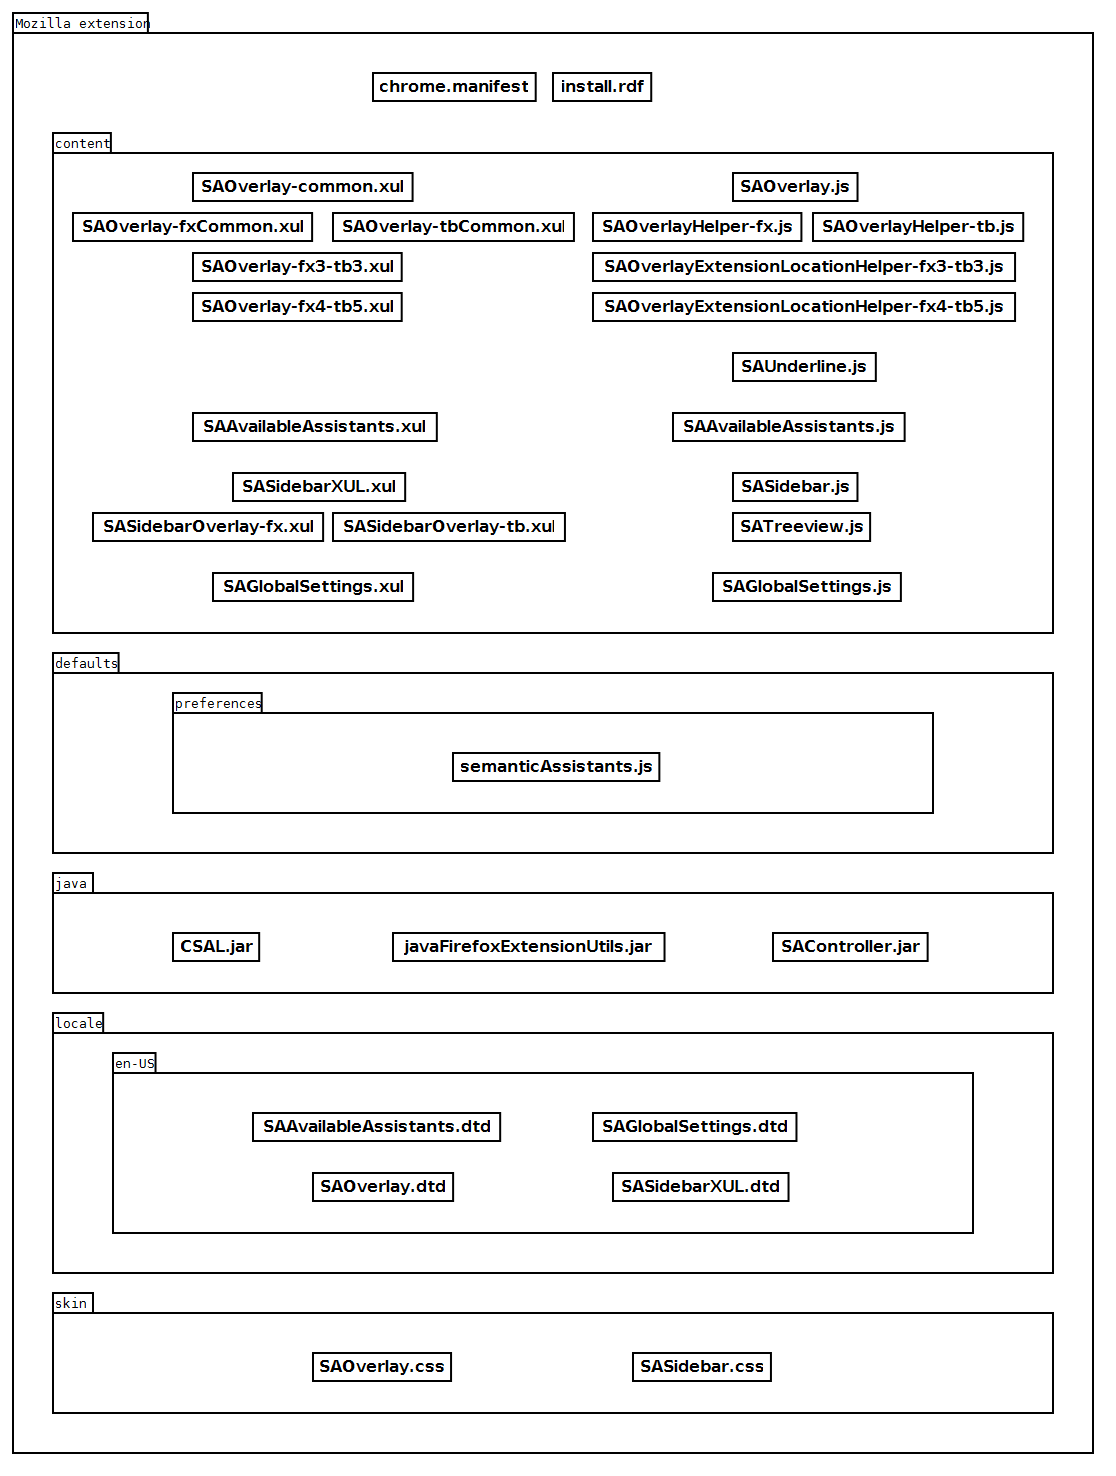
\includegraphics[totalheight=0.8\textheight]{pictures/mozilla_development_notes_file_layout.png}
  \caption{The file layout of the Mozilla extension}
  \label{fig:mozilla_development_notes_file_layout}
\end{figure}

\paragraph{Root folder} At the root of extension folder are two files called ``chrome.manifest" and ``install.rdf". The ``chrome.manifest" identifies the files contained within the extension and also allows to specify which files of the extension are to be loaded, depending on the application and the version of the application on which the extension is running (more on this later). The ``install.rdf" file defines various information about the extension, including the name of the extension (which becomes the name of the aforementioned extension folder), which applications and application versions that the extension is compatible with, and so on. 
\paragraph{The ``content" folder} This contains a series of XUL (.xul) files and JavaScript (.js) files. The XUL files define the user interface elements and behavior, such as windows, dialogs, menus, toolbar buttons. The JavaScript files contain the execution logic, and manipulation of user interface elements. 
\paragraph{The ``defaults" folder} Within the ``defaults" folder is the ``preferences" folder, which contains the default preferences for the extension. Upon installation of the extension, these defaults are set as the preferences in the Firefox/Thunderbird user profile (see above for specifics about preferences). 
\paragraph{The ``java" folder} The ``java" folder contains precompiled Java classes contained within .jar files. The ``CSAL.jar" is the same Client Side Abstraction Layer found in other clients. The ``javaFirefoxExtensionUtils.jar" file is a third-party utility which allows to grant full privileges to Java within a Mozilla extension. The ``SAController.jar" file is the Java component of the extension, which acts as a bridge between the JavaScript code and the CSAL and contains some additional execution logic. 
\paragraph{The ``locale" folder} The purpose of the ``locale" folder is to contain folders that contain files with localized strings used within the extension. These folders are named by specific languages' abbreviations (e.g., ``en-US"). 
\paragraph{The ``skin" folder} The ``skin" folder contains .css files that define layout and appearance properties image resource files for the icons and various UI elements within the extension.

\subsection{Compatibility Concerns}
There are differences in the extension between Firefox and Thunderbird. Furthermore, such differences also exist between Firefox 3.6.x and Firefox 4.0 as well as between Thunderbird 3.1.x and Thunderbird 5.0. (There was no Thunderbird 4.0.) This was because major changes were made to the Mozilla platform between those versions of the appliations. 

In order to enable the extension to be compatible with multiple version of Firefox as well as multiple versions of Thunderbird, certain measures were taken. 

Files of the extensions were split such that common code between applications/versions are kept within common files, while code that is different between applications/versions are separated into different versions of the files. The appropriate set of files is loaded for the right application and version. 

The aforementioned ``chrome.manifest" file, located at the root of the extension's folder structure, specifies the files to be loaded for the extension, depending on the application and application version on which the extension is running. Hence, for example, this allows for one file to be loaded for Firefox and another file to be loaded for Thunderbird. Another example would be for one file to be loaded for Firefox version 3.6 and earlier and another file to be loaded for Firefox version 4 and later. 

The files that need to have multiple versions are both the JavaScript files and the XUL files. The JavaScript code may differ between applications/versions due to differences in API. XUL files differ between applications (less for between versions of the same application) due to differences in the user interfaces (different elements, different naming, etc.).

Table~\ref{tab:mozilla_development_files_compatibility} shows which files are used depending on the application and the version of the application. 

\begin{table}[htb]
  \centering\small\sffamily
  \begin{tabular}{p{0.5\textwidth}@{\hspace*{4mm}}p{0.08\textwidth}@{\hspace*{4mm}}p{0.08\textwidth}@{\hspace*{4mm}}p{0.08\textwidth}@{\hspace*{4mm}}p{0.08\textwidth}}
    \toprule
    \textbf{} & \textbf{Fx 3.6.x} & \textbf{Fx 4.0+} & \textbf{Tb 3.1.x} & \textbf{Tb 5.0+} \\
    \midrule
    SAOverlay.js & x & x & x & x \\

    SAOverlayHelper-fx.js & x & x &  &  \\

    SAOverlayHelper-tb.js &  &  & x & x \\

    SAOverlayExtensionLocationHelper-fx3-tb3.js & x &  & x &  \\

    SAOverlayExtensionLocationHelper-fx4-tb5.js &  & x &  & x \\

    SAOverlay-common.xul & x & x & x & x \\

    SAOverlay-fxCommon.xul & x & x &  &  \\

    SAOverlay-tbCommon.xul &  &  & x & x \\

    SAOverlay-fx3-tb3.xul & x &  & x &  \\

    SAOverlay-fx4-tb5.xul &  & x &  & x \\

    SASidebarXUL.xul & x & x & x & x \\

    SASidebarOverlay-fx.xul & x & x &  &  \\

    SASidebarOverlay-tb.xul &  &  & x & x \\
    \bottomrule
  \end{tabular}
  \caption{Files loaded depending on application and version for compatibility}
  \label{tab:mozilla_development_files_compatibility}
\end{table}

\subsection{Extension Preferences}
The default preferences of the extension are defined in the folder ``defaults" in the ``preferences" subfolder in the file ``semanticAssistants.js". As previously mentioned, the current settings of those preferences are stored in a file called ``prefs.js" in the user profile folder. 

The preferences are: 

\begin{itemize}
  \item \emph{extensions.semanticAssistants.firstTimeRun} \begin{itemize}
    \item type: boolean
    \item default value: true
    \item This determines whether it is the first time that the extension is launched. If so, it adds the toolbar menu button to the application's main toolbar. 
  \end{itemize}
  \item \emph{extensions.semanticAssistants.installLocation} \begin{itemize}
    \item type: string
    \item default value: ""
    \item This stores the path of the extension. This is not a user preference; it is utilized internally when accessing the .jar files. It is set in the extension when the application's start up. 
  \end{itemize}
  \item \emph{extensions.semanticAssistants.serverCustomHost} \begin{itemize}
    \item type: string
    \item default value: ""
    \item This is a setting set by the user in the ``Global Settings" dialog. 
  \end{itemize}
  \item \emph{extensions.semanticAssistants.serverCustomPort} \begin{itemize}
    \item type: string
    \item default value: "8879"
    \item This is a setting set by the user in the ``Global Settings" dialog. 
  \end{itemize}
  \item \emph{extensions.semanticAssistants.serverDefaultOrCustom} \begin{itemize}
    \item type: integer
    \item default value: 0
    \item 0 for ``Default", 1 for ``Custom"
    \item This is a setting set by the user in the ``Global Settings" dialog. 
  \end{itemize}
\end{itemize}

\subsection{Overall Architecture}
The Mozilla extension is composed of three components: the principal component in JavaScript and XUL, the Java component of the extension (contained in the aforementioned ``SAController.jar" file), and the Client Side Abstraction Layer/CSAL (the ``CSAL.jar" file). A high-level representation of the overall architecture is shown in Figure~\ref{fig:mozilla_development_notes_overall_architecture_high_level}).
The main part of the extension is in JavaScript and XUL, as extensions for the Mozilla platform are written in JavaScript code, and the user interface is defined in XUL. A Java component exists in order for the JavaScript component to interoperate with the CSAL; it also adds additional execution logic, such as processing the results from the CSAL. Leveraging a feature in Firefox/Thunderbird called LiveConnect in addition to a third-party package to grant full privileges to Java within a Mozilla extension, the JavaScript code of the extension utilizes and calls the compiled Java code, which in turn utilizes and calls the CSAL. 

\begin{figure}[htb]
  \centering
  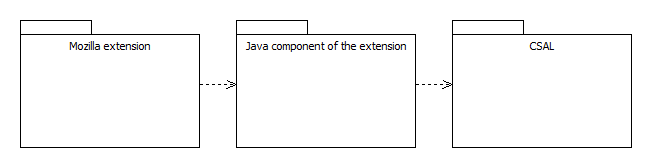
\includegraphics[width=0.8\textwidth]{pictures/mozilla_development_notes_overall_architecture_high_level.png}
  \caption{The overall architecture of the Mozilla extension at a high level}
  \label{fig:mozilla_development_notes_overall_architecture_high_level}
\end{figure}

The main class in the Mozilla extension component is ``SAOverlay" (defined in ``SAOverlay.js" under the ``contents" folder). This class communicates with the other classes in the component. Additionally, it is this class that calls the Java component. The facade for the Java component is the ``SemanticAssistantsController" class. Similarly, the ``SemanticAssistantsController" class is a controller, which coordinates the other classes in the Java component. The various classes of the Java component utilize classes contained within the CSAL. These dependencies are shown in Figure~\ref{fig:mozilla_development_notes_overall_architecture_more_detailed}.

\begin{figure}[htb]
  \centering
  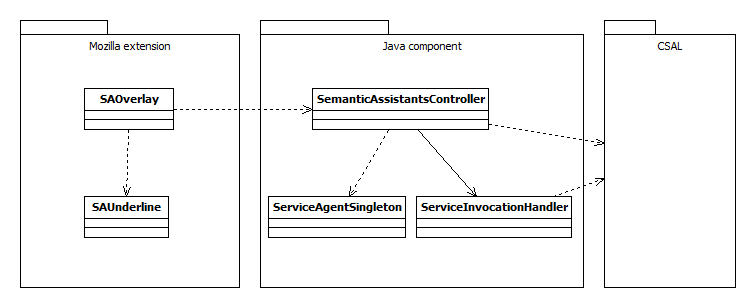
\includegraphics[width=0.8\textwidth]{pictures/mozilla_development_notes_overall_architecture_more_detailed.png}
  \caption{The overall architecture of the Mozilla extension showing some more details in terms of dependencies and showing some of the main modules}
  \label{fig:mozilla_development_notes_overall_architecture_more_detailed}
\end{figure}

\subsection{Main Mozilla Extension Component}
The main component of the Mozilla extension consists of a series of JavaScript classes and XUL files. The class diagram in Figure~\ref{fig:mozilla_development_notes_mozilla_extension_class_diagram} shows the main classes and their associations in the main Mozilla extension component as well as the classes called within the Java component. 

\begin{figure}[htb]
  \centering
  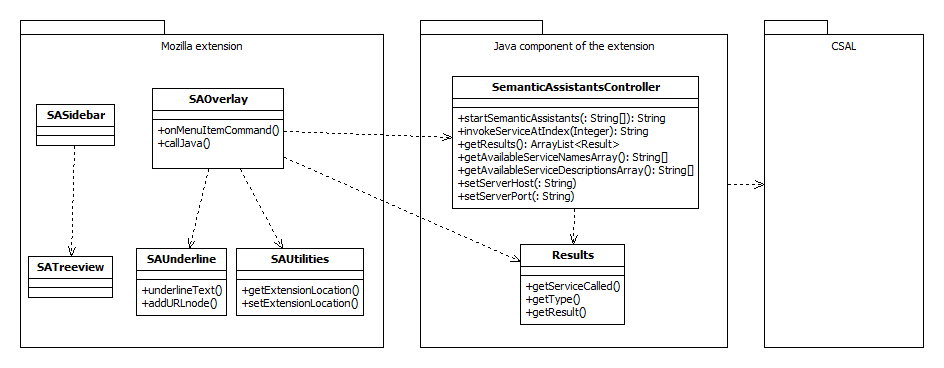
\includegraphics[width=0.95\textwidth]{pictures/mozilla_development_notes_mozilla_extension_class_diagram.png}
  \caption{Class diagram of the main Mozilla extension component}
  \label{fig:mozilla_development_notes_mozilla_extension_class_diagram}
\end{figure}

The main class is ``SAOverlay". When the user invokes the ``Available Assistants" command, it invokes the ``onMenuItemCommand" function in ``SAOverlay". This function obtains the user selection on the page/message, or the whole content of the page/message if no selection was made, and calls the function ``callJava" and passes the user selection. The ``callJava" function then obtains references to the Java classes in the Java component (``SAController.jar"). This is done using the feature called LiveConnect built into Firefox and Thunderbird. Additionally, the aforementioned third-party component ``javaFirefoxExtensionUtils.jar" is required to grant full privileges to the .jar files, as shown in Figure~\ref{list:mozilla_development_notes_main_mozilla_extension_component_jar_permissions}. The method ``startSemanticAssistants" of the ``SemanticAssistantsController" Java class is invoked, and the result returned is a list of available \sa NLP services (``Assistants"). Then, an XUL dialog ``SAAvailableAssistants.xul" is opened, prompting the user to choose an Assistant from the list. 

\begin{figure}
\centering
\begin{lstlisting}[language=Java,numbers=left,xleftmargin=4mm,columns=flexible]
callJava: function(userSelection, allText) {
    var extensionPath = SAOverlay.getExtensionLocation();
    
    var SAControllerJarPath = "file:///" + extensionPath + "/java/SAController.jar"; 
    var classLoaderJarPath = "file:///" + extensionPath + "/java/javaFirefoxExtensionUtils.jar";
    var CSALJarPath = "file:///" + extensionPath + "/java/CSAL.jar";
    
    urlArray = []; 
    urlArray[0] = new java.net.URL(SAControllerJarPath); 
    urlArray[1] = new java.net.URL(classLoaderJarPath);  
    urlArray[2] = new java.net.URL(CSALJarPath);  

    var cl = java.net.URLClassLoader.newInstance(urlArray);

    //set security policies with the policyAdd function defined below
    this.policyAdd(cl, urlArray);
    
    (...)
}, 

(...)

policyAdd: function(loader, urls) {
    try {
        var str = 'edu.mit.simile.javaFirefoxExtensionUtils.URLSetPolicy';
        var policyClass = java.lang.Class.forName(
            str,
            true,
            loader
            );
        var policy = policyClass.newInstance();
        policy.setOuterPolicy(java.security.Policy.getPolicy());
        java.security.Policy.setPolicy(policy);
        policy.addPermission(new java.security.AllPermission());
        for (var j = 0; j < urls.length; j++) {
            policy.addURL(urls[j]);
        }
    }
    catch(e) {
        alert(e+'::'+e.lineNumber);
    }
}
\end{lstlisting}
\caption{Granting full permissions to .jar files inside the extension in the \texttt{callJava} function in the \texttt{SAOverlay} class}
\label{list:mozilla_development_notes_main_mozilla_extension_component_jar_permissions}
\end{figure}

When the selection is made, another method ``invokeServiceAtIndex" of the ``SemanticAssistantsController" Java class is invoked, and upon successful return of the results, the ``getResults" method of the Java class is called to retrieve the results from the service invocation. Then, for each result within the results, an appropriate action is taken. For an ``annotation"-type result, the function ``underlineText" of the ``SAUnderline" JavaScript class is called; for a ``document"-type result, the function ``addURLnode" of ``SAUnderline" is called; for a ``file"-type result, no action is taken, as the Java code executes the opening the file. Save for a ``file"-type result, the ``Semantic Assistants" sidebar, which is the XUL file ``SASidebarXUL.xul", is opened to display the results. 

The sequence diagram in Figure~\ref{fig:mozilla_development_notes_mozilla_extension_sequence_diagram_main_scenario} shows the call sequence involved in the above main scenario of listing the available services and then of invoking a service. 
\begin{figure}[htb]
  \centering
  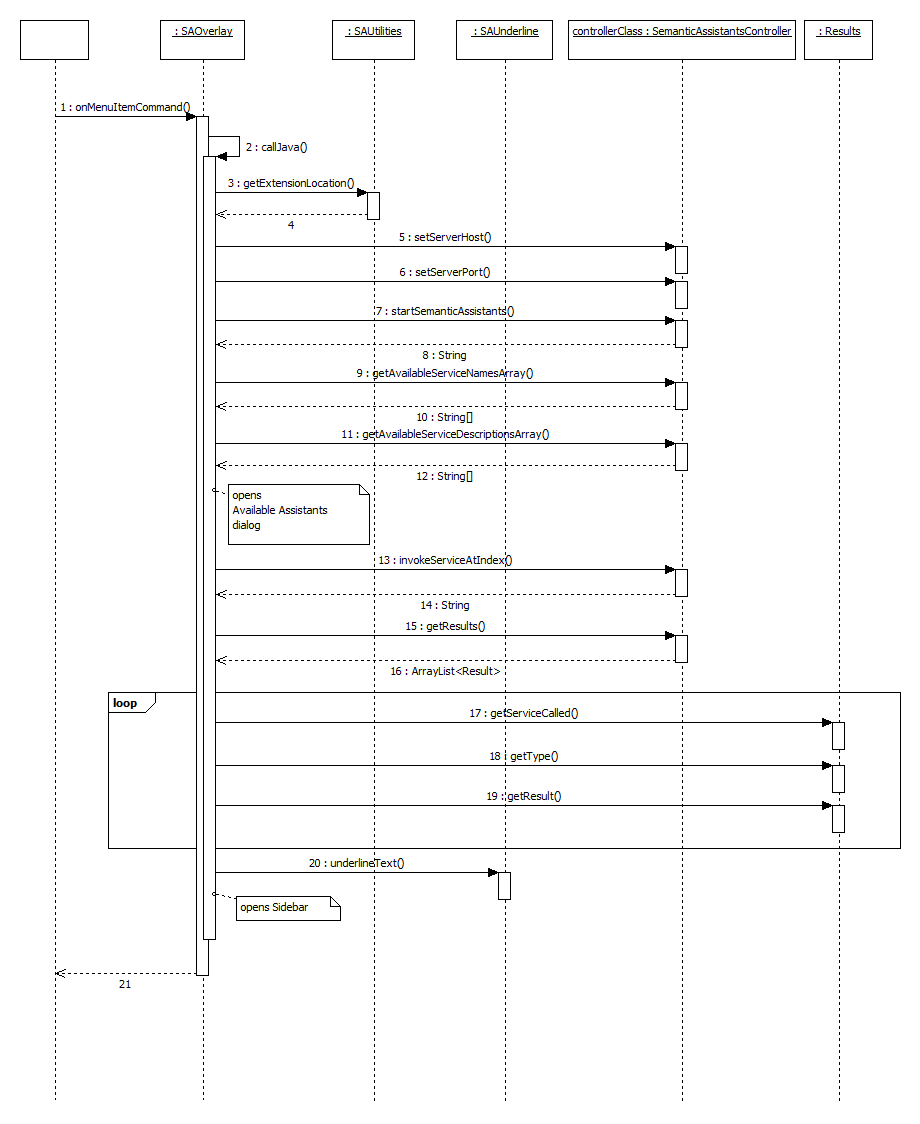
\includegraphics[totalheight=0.8\textheight]{pictures/mozilla_development_notes_mozilla_extension_sequence_diagram_main_scenario.png}
  \caption{Sequence diagram of the main Mozilla extension component for the main scenario}
  \label{fig:mozilla_development_notes_mozilla_extension_sequence_diagram_main_scenario}
\end{figure}

\subsection{Java Component}
The Java component consists of a series of Java classes packaged within a .jar file. The class diagram in Figure~\ref{fig:mozilla_development_notes_java_component_class_diagram} shows the principal classes and their associations in the Java component as well as some of the classes in the CSAL called from the Java component. 

\begin{figure}[htb]
  \centering
  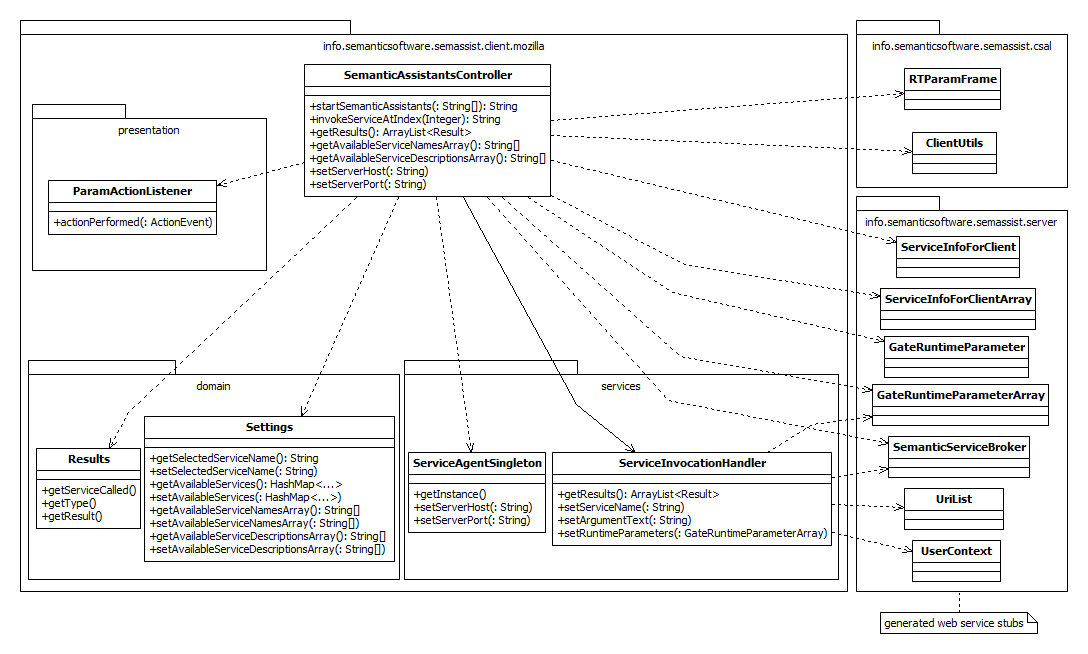
\includegraphics[width=0.95\textwidth]{pictures/mozilla_development_notes_java_component_class_diagram.png}
  \caption{Class diagram of the Java component}
  \label{fig:mozilla_development_notes_java_component_class_diagram}
\end{figure}

The main class is ``SemanticAssistantsController"; it is the facade class of the Java component packaged within ``SAController.jar" file and acts as a controller that calls and coordinates all other classes. 

\paragraph{The scenario of getting available services} The method ``startSemanticAssistants" of the ``SemanticAssistantsController" class is called. By calling ``getInstance" of ``ServiceAgentSingleton", a ``SemanticServiceBroker" instance is obtained. Calling ``getAvailableServices" of the latter returns a ``ServiceInfoForClientArray", which is a collection of the available services from the server. Then, these available services are stored in the ``Settings" class, as well as service names and service descriptions to be utilized by the main JavaScript component to display to the user. (A code snippet of this can be seen in Figure~\ref{list:mozilla_development_notes_java_component_get_available_services}.)

The sequence diagram in Figure~\ref{fig:mozilla_development_notes_java_component_sequence_diagram_get_available_services} shows the call sequence in the above scenario of obtaining the list of available services from the server. 

\begin{figure}
\centering
\begin{lstlisting}[language=Java,numbers=left,xleftmargin=4mm,columns=flexible]
SemanticServiceBroker agent = ServiceAgentSingleton.getInstance();
ServiceInfoForClientArray sia = agent.getAvailableServices();

List<ServiceInfoForClient> results = sia.getItem();
Iterator<ServiceInfoForClient> it = results.iterator();

(...)

while( it.hasNext() ) {
    ServiceInfoForClient info = it.next();
    availableServices.put( info.getServiceName(), info );
    (...)
}

(...)

Settings.setAvailableServices( availableServices );
\end{lstlisting}
\caption{Getting the available services in the the \texttt{startSemanticAssistants} method in the \texttt{SemanticAssistantsController} class}
\label{list:mozilla_development_notes_java_component_get_available_services}
\end{figure}

\begin{figure}[htb]
  \centering
  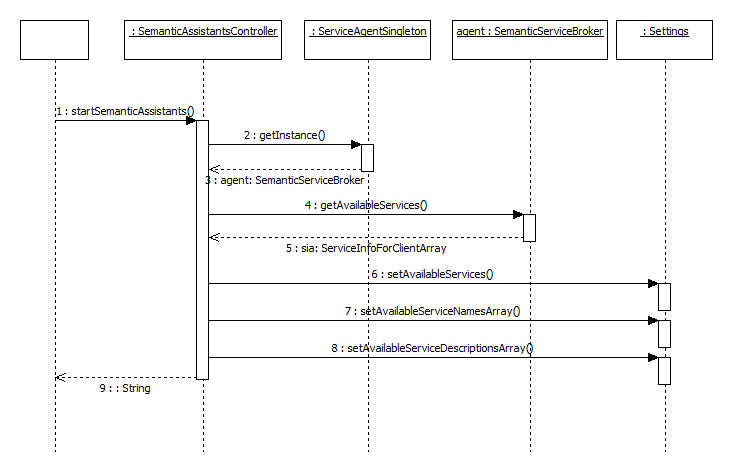
\includegraphics[width=0.95\textwidth]{pictures/mozilla_development_notes_java_component_sequence_diagram_get_available_services.png}
  \caption{Sequence diagram of the Java component for the scenario of getting available services}
  \label{fig:mozilla_development_notes_java_component_sequence_diagram_get_available_services}
\end{figure}

\paragraph{The scenario of invoking an available service} The method ``invokeServiceAtIndex" of the ``SemanticAssistantsController" class is called with the argument passed from the JavaScript code specifying which service was specified by the user. The name of the service, which is what is used to identify services, is determined. The method ``runSelectedService" is called, where the ``ServiceInfoForClient" corresponding to the service is retrieved from the list saving during the ``startSemanticAssistants" method call. 

If this service has parameters to be entered by the user, these parameters are retrieved based on the service and displayed in a ``JFrame" for the user to enter the required and optional parameters. 

A new ``GateRuntimeParameterArray" instance, containing the user input for the parameters if there were any, is passed to ``doRunSelectedService" method. In this method, the service name and text to be analyzed are set in a newly instantiated ``ServiceInvocationHandler" is instantiated, then ``getResults" is called. In this method, from ``ServiceAgentSingleton", ``SemanticServiceBroker" instance is obtained; ``invokeService" of this instance is called upon while passing the service name, the text to be analyzed, the parameters (if any), as well as other arguments. The result returned is a string which when processed by the ``getServiceResults" method of ``ClientUtils" yields a list of ``SemanticServiceResult" results. Then, each result is processed according to its result type. For example, for a "file"-type result, code is run to open the file in the Web browser; for a "annotation"- or "document"-type result, the result is set appropriately in the list of results returned to the JavaScript code, to be then processed by the main extension component. 

The sequence diagram in Figure~\ref{fig:mozilla_development_notes_java_component_sequence_diagram_invoke_service} shows the call sequence in the above scenario of invoking an available service from the server and obtaining the results. 

\begin{figure}[htb]
  \centering
  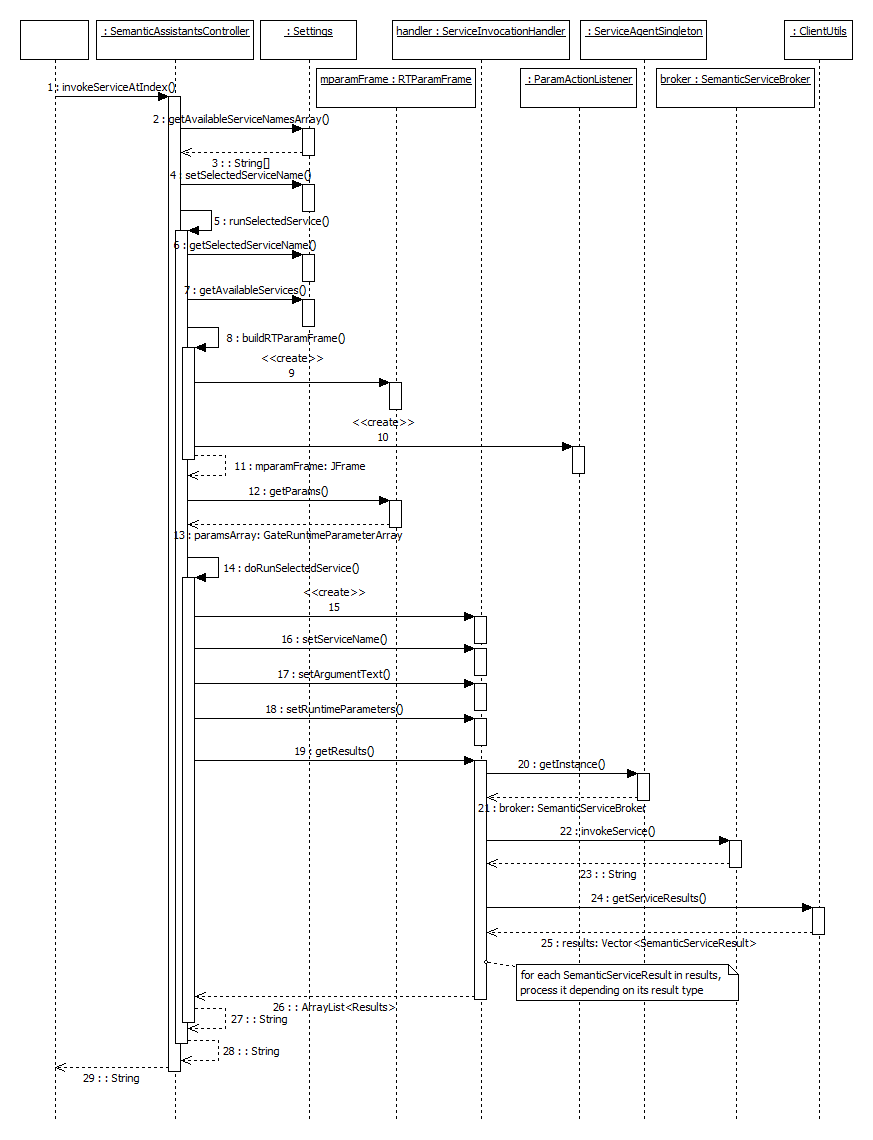
\includegraphics[totalheight=0.8\textheight]{pictures/mozilla_development_notes_java_component_sequence_diagram_invoke_service.png}
  \caption{Sequence diagram of the Java component for the scenario of invoking a service}
  \label{fig:mozilla_development_notes_java_component_sequence_diagram_invoke_service}
\end{figure}
